\documentclass[runningheads,a4paper]{llncs}
\usepackage{color}
\usepackage{amssymb}
\setcounter{tocdepth}{3}
\usepackage{graphicx}
\usepackage{framed}
\usepackage{url}
\usepackage{float}
\urldef{\mailsa}\path|firstname.lastname@gesis.org|
\newcommand{\keywords}[1]{\par\addvspace\baselineskip
\noindent\keywordname\enspace\ignorespaces#1}

\begin{document}

\mainmatter  % start of an individual contribution

% first the title is needed
\title{Analyzing the research output presented at European Networked Knowledge Organization Systems workshops (2000-2015)}

% a short form should be given in case it is too long for the running head


% the name(s) of the author(s) follow(s) next
%
% NB: Chinese authors should write their first names(s) in front of
% their surnames. This ensures that the names appear correctly in
% the running heads and the author index.
%
\author{Fakhri Momeni%
	\and Philipp Mayr}
%
\titlerunning{Analyzing the NKOS research output (2000-2015)}
% (feature abused for this document to repeat the title also on left hand pages)

% the affiliations are given next; don't give your e-mail address
% unless you accept that it will be published
\author{Fakhri Momeni and Philipp Mayr}
\institute{GESIS - Leibniz Institute for the Social Sciences,\\
	Unter Sachsenhausen 6-8\\
	50667 Cologne, Germany\\
	\email{firstname.lastname@gesis.org} }

%
% NB: a more complex sample for affiliations and the mapping to the
% corresponding authors can be found in the file "llncs.dem"
% (search for the string "\mainmatter" where a contribution starts).
% "llncs.dem" accompanies the document class "llncs.cls".
%

%\toctitle{Lecture Notes in Computer Science}
%\tocauthor{Authors' Instructions}
\maketitle


\begin{abstract}		
In this paper we analyze a major part of the research output of the Networked Knowledge Organization Systems (NKOS) community in the period 2000 to 2015 from a network analytical perspective. We focus on the paper output presented at the European NKOS workshops in the last 15 years. Our open dataset, the "NKOS bibliography", includes 14 workshop agendas (ECDL 2000-2010, TPDL 2011-2015) and 4 special issues on NKOS (2001, 2004, 2006 and 2015) which cover 171 papers with 218 distinct authors in total. A focus of the analysis is the visualization of co-authorship networks in this interdisciplinary field. We used standard network analytic measures like degree and betweenness centrality to describe the co-authorship distribution in our NKOS dataset.  We can see in our dataset that 15\% (with degree=0) of authors had no co-authorship with others and 53\% of them had a maximum of 6 cooperations with other authors. 32\% had at least 8 co-authors for all of their papers. In general we see an average of 1.9 authors for a workshop paper and 2.3 authors for a special issue journal paper.

 
\keywords{European NKOS workshops, Output analysis, Network analysis, Central authors, Collaboration}
\end{abstract}


\section{Introduction}\label{intro}

The European NKOS network has held a long-running series of annual workshops at the European Conference on Digital Libraries (ECDL), latterly reformed as the International Conference on Theory and Practice of Digital Libraries (TPDL). 
Typically, recent advances of KOS have been reported at the NKOS workshops, e.g. including the Simple Knowledge Organization System (SKOS) W3C standard, the ISO 25964 thesauri standard, the CIDOC Conceptual Reference Model (CRM), Linked Data applications, KOS-based recommender systems, KOS mapping techniques, KOS registries and metadata, social tagging, user-centred issues, and many other topics. A comprehensive and well cited review article on KOS and NKOS topics was published in 2004 \cite{Zeng2004}. Special issues on Networked Knowledge Organization Systems (NKOS) have been published in Journal of Digital Information in 2001 and 2004, in New Review of Hypermedia and Multimedia in 2006 and recently in International Journal of Digital Libraries in 2015 \cite{Mayr2016}. 

The motivation of this paper is to analyze the research output of the NKOS community. We are focusing on the informal part of this output, the paper presentations given at the past NKOS workshops (the first European NKOS workshop in 2000 to the 14th European NKOS workshop in 2015). The specialty of this research output is that these research papers typically are not published in journals or conference proceedings. These papers appear just as oral presentations at the workshop and are documented on the website. 

To our knowledge nobody has done an analysis on this part of the NKOS research output before. 



\section{NKOS workshop bibliography}\label{dataset}

For our analysis we have compiled an open dataset the "NKOS bibliography"\footnote{The NKOS workshop bibliography is maintained in the following github repository: https://github.com/PhilippMayr/NKOS-bibliography} which includes 14 workshop programs with all presented papers at ECDL 2000, ECDL 2003-2010 and TPDL 2011-2015 (see Table \ref{tab:workshops}). We added papers from 4 special issues on NKOS which have been edited by members of the NKOS community in the same period (see Table \ref{tab:SI}). 

In a first step we have extracted all paper titles presented at the NKOS workshop websites. We excluded welcome and introduction presentations. We added journal papers from the four mentioned special issues on NKOS. These journal papers are the only formal publications in our analysis. In the end we manually disambiguated author names of all papers.

Our dataset covers 171 papers in total with a sum of 218 distinct author names. Table \ref{tab:workshops} provides an overview of all workshop papers\footnote{See readme for details on the workshops under https://github.com/PhilippMayr/NKOS-bibliography/blob/master/readme.txt}. We can see a slightly decreasing amount of papers presented at the workshops after ECDL has renamed to TPDL in 2011. In average 1.9 authors published a workshop paper.

\begin{table}
	\centering
	\caption{Overview of all NKOS workshop papers}
\begin{tabular}	{|c|c|c|}		
	\hline 
	venue& papers  & authors  \\ 
	\hline 
	ECDL 2000& 4 & 4 \\ 
	\hline 
	ECDL 2003& 13 & 11 \\ 
	\hline 
	ECDL 2004& 14 & 27 \\ 
	\hline 
	ECDL 2005& 12 & 26 \\ 
	\hline 
	ECDL 2006& 12 & 27 \\ 
	\hline 
	ECDL 2007& 15 & 26 \\ 
	\hline 
	ECDL 2008& 11 & 16 \\ 
	\hline 
	ECDL 2009& 12 & 31 \\ 
	\hline 
	ECDL 2010& 12 & 25 \\ 
	\hline 
	TPDL 2011& 11 & 26 \\ 
	\hline 
	TPDL 2012& 9 & 22 \\ 
	\hline 
	TPDL 2013& 7 & 17 \\ 
	\hline 
	TPDL 2014& 9 & 17 \\ 
	\hline 
	TPDL 2015& 7 & 13 \\ 
	\hline 
\end{tabular} 
\label{tab:workshops}
\end{table}

Table \ref{tab:SI} provides an overview of all papers in the special issues. We can see that a relative constant number of papers in the issues have an increasing number of authors. In average 2.3 authors published a special issue journal paper.

\begin{table}
	\centering
	\caption{Overview of all NKOS special issue papers}
\begin{tabular}{|c|c|c|}  
	\hline 
	venue& papers  & authors  \\ 
	\hline 
	JODI 2001 \cite{Hill2001} & 5 & 8 \\ 
	\hline 
	JODI 2004 \cite{Tudhope2004} & 5 & 15 \\ 
	\hline 
	NREV 2006 \cite{Tudhope2006} & 6 & 11 \\ 
	\hline 
	IJDL 2015 \cite{Mayr2016} & 7 &  20\\ 
	\hline 
\end{tabular} 
\label{tab:SI}
\end{table}

%Check the citation counts of the SI papers in WoS/Google scholar.  


\section{Analysis}\label{analysis}

In order to analyze the collaboration of the NKOS community we built a network of all authors at the workshops and special issues and computed the centrality of each author. For this purpose we utilized some standard centrality measures in Pajek\footnote{A program for analysis and visualization of very large networks (http://mrvar.fdv.uni-lj.si/pajek/)}. The network is composed of pairs of author names. Each pair means that two authors cooperated for writing a paper. If we have n papers and the paper \textit{i} has $m_i$ authors, the number of pairs are 

\begin{equation}\sum\limits_{i=1}^n \frac{m_i(m_i-1)}{2}\end{equation}

These pairs built the network for our analysis in Pajek. To avoid repetition of pairs, we gave weight to pairs and this is equal to the number of cooperations of two authors in different papers. 
Two often used centrality measures of authors are degree and betweenness. Degree is the number of nodes that a focal node is connected to and measures the involvement of the node in the network \cite{Opsahl2010}. In our authorship-network it specifies the sum of co-authors for all papers that each author has written. Betweenness assesses the degree to which a node lies on the shortest path between two other nodes and is able to funnel the flow in the network \cite{Opsahl2010}. In the authorship-network the author with a high betweenness has a large influence on the transfer of information. 


\section{Results}\label{results}

Figure \ref{fig:wholenet} demonstrates a general view of the network. In this view each author has at least one co-author. This network contains 31 components. From the network illustrated in this figure we selected the largest component that is represented in Figure \ref{fig:largestComponent}. 68 authors (31\% of all authors) are connected in this component. 
%todo Fakhri check number
From figure \ref{fig:wholenet} we see that 58 authors (27\%) had just one paper.


\begin{figure}
	\centering
	\includegraphics[width=1.0\linewidth]{wholeNet}
	\vspace{-0.5em}
	\caption{Network of authors in the European NKOS community}
	\label{fig:wholenet}
	\vspace{-0.5em}
\end{figure}

%todo add some more details and interpretation; Peter fragen

\begin{figure}[H]
	\centering
	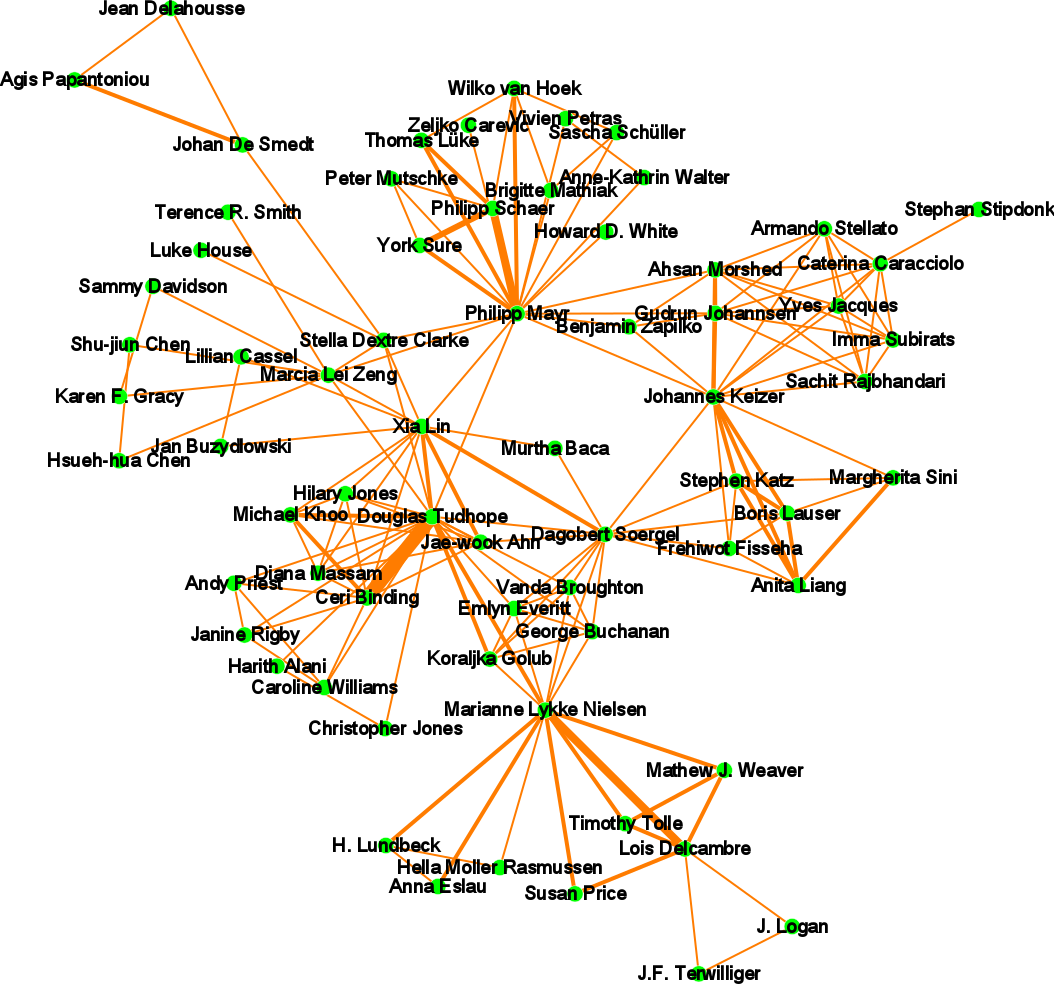
\includegraphics[width=0.9\linewidth]{largestComponent}
	\caption{Largest component in the NKOS authorship-network}
	\label{fig:largestComponent}
\end{figure}

To show the quantity of collaboration in the community we measured the degree centrality for each author. Figure \ref{fig:degreePercentage} shows the percentage of authors with different degrees. In this figure we see that 15\% (with degree=0) of authors had no co-authorship with others and 53\% of them had a maximum of 6 cooperations with other authors. 32\% had at least 8 co-authors for all their papers.

%todo add some more details and interpretation

\begin{figure}[H]
	\centering
	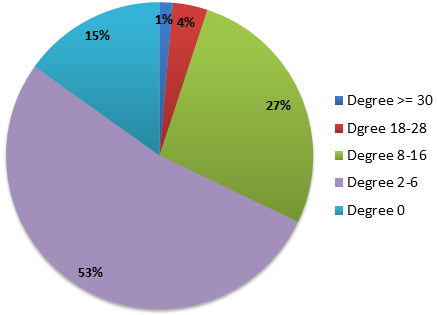
\includegraphics[width=0.6\linewidth]{degreePercentage}
	\caption{Distribution of degree numbers of authors in the network} 
	\label{fig:degreePercentage}
\end{figure}

Figure \ref{fig:degree16} shows the authors with high degree (more than 16) in the network. 

\begin{figure}[H]
	\centering
	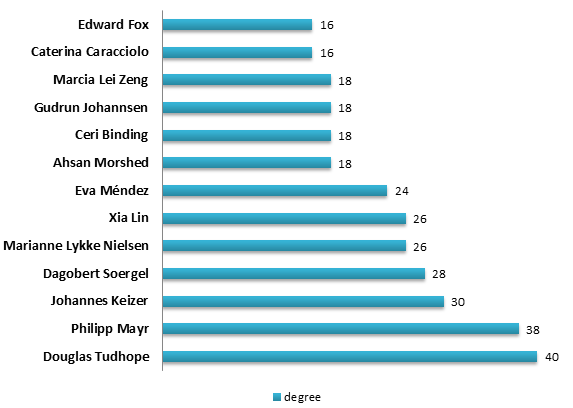
\includegraphics[width=0.8\linewidth]{degree16}
	\caption{Authors with degree more than 16}
	\label{fig:degree16}
\end{figure}


To detect the influence of authors on information exchange we calculated the betweenness centrality of authors. Figure \ref{fig:betweenness} indicates the authors with high betweenness (more than 0.001). If we compare betweenness with degree we can see that the ranking of authors has changed. We observe that some authors have lower ranking in betweenness (despite their high cooperation with other authors) in comparison to others with lower degree. 

%todo add some more details and interpretation

\begin{figure}
\centering
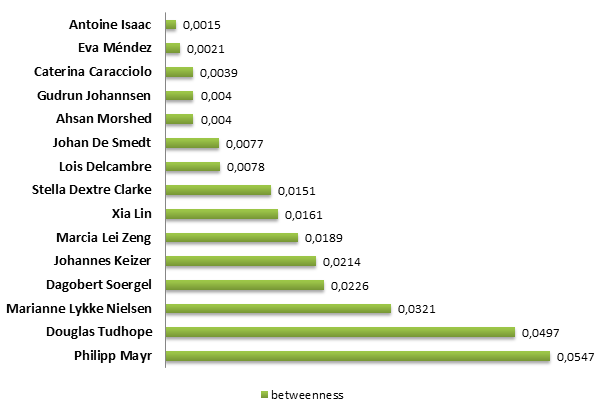
\includegraphics[width=0.8\linewidth]{betweenness}
\caption{Authors with betweenness more than 0.001}
\label{fig:betweenness}
\end{figure}


\section{Conclusion}\label{concl}
In this paper we have started to analyze the collaborative research of authors and their connectivity to each other in the special case of European NKOS workshop activities and four special issues on NKOS. The results show most active authors in this community who had an important role in the exchange of information exchange and in connecting researchers. We saw some details of the largest component in this network that covers one third of the authors of the whole network. Our analyses show that NKOS workshops were pretty successful in bringing researchers together.  

%todo add some interpretation

We know that our dataset has some severe limitations. 
First of all we have included just paper presentations. Editing and organizing activities at the workshops have not been covered in our dataset. This leads to artifacts; e.g. Traugott Koch,\footnote{Traugott Koch was an important protagonist and networker of the European NKOS community. He retired and left the NKOS community in 2012.} a long-term organizer of the NKOS workshops and editor of the early JoDI special issues on NKOS, is not included in our dataset and the network. 

Second, we have not included the activities of the NKOS community in the United States of America. The website at Kent State\footnote{http://nkos.slis.kent.edu/} would be a great starting point to look up more research activities of the US NKOS community.

Third, we have not included bibliometric data to complete our analysis. This is because most of the NKOS workshop activities (presentations) are not formally cited or even mentioned in scientific papers. In difference to the workshop output, the few journal papers in the special issues on NKOS are cited. Some works (e.g. \cite{SPCranefield2001,SPDoerr2001,SPTudhope2001,SPSoergel2004,SPTrant2006}) are cited well in the literature. 

%Table xy lists papers of the special issue from 2001, 2004 and 2006 and their citation counts shown in Google Scholar.


\section{Future work}\label{future}
We are planning to extend the analysis of the NKOS network. In this way we first plan to complement the dataset with other NKOS research output. We also plan to analyze the development of topics in the titles and abstracts of the presentations and papers. Combining network analytic measures with bibliometric analysis (e.g. co-citations, bibliographic coupling) would complement our preliminary observations.

\section{Acknowledgment}\label{sec:ACKNOWLEDGMENTS}
We thank our colleague Julia Achenbach (GESIS) who helped us to compile and correct the dataset.

\newpage

\bibliographystyle{splncs03} % abbrev
\bibliography{nkos} 

\end{document}
